\documentclass[12pt]{article}
\usepackage{graphicx}
\usepackage{fullpage}
\usepackage{float}
\usepackage{hyperref}

\title{Writeup - Author Identification}
\author{Lev Teytelman}
\date{\today}

\begin{document}\maketitle
\section{Introduction}
This assignment finds authors with the most similar writing styles. The program takes a number of command-line flags to specify the database of texts to use, the noise file to read in, the number of closest matches to print out, the number of words to parse in from the noise file, and flags to set the distance formula. I also added a flag to enable verbose mode to see the number of hashes, hash table lookups, and Bloom filter lookups. It then opens the texts from the database and compares them to the one given through standard input by comparing the normalized text frequencies, sorts the calculated distances and authors, and outputs the top $k$ authors/distances as specified.

\section{The Hash Function}
While the SPECK cipher is cryptographically secure, it is very slow for our case. Therefore, I replaced it with a faster function that gave a good distribution while speeding up the program drastically. This function was inspired by Elmer's experimentation with hash functions in Discord, where I changed some aspects and experimented until I found a good balance of speed and random distribution. Comparing the two hash functions, we can see that the modified one is faster, but has slightly more collisions than the SPECK function (no collisions would mean exactly one probe per insertion or lookup):
\begin{verbatim}
SPECK Cipher
Average Probes per Insertion: 1.009002
Average Probes per Lookup: 1.025079
Seconds taken: 31.599

Modified Hashing Function
Average Probes per Insertion: 1.012787
Average Probes per Lookup: 1.040532
Seconds taken: 19.327
\end{verbatim}
I used \verb|hyperfine| as suggested by Eugene to find the average runtime the programs over 10 runs. As seen by the statistics, there are slightly more collisions with the faster hash function. However, the increased speed of the function outweighs the increased number of collisions and speeds the program up by nearly two times.

\section{Size of the Hash Table}
After speeding up the program with a faster hashing function, I turned my attention to the hash table. By changing just the size of the hash table, I was able to see a direct correlation between its size in memory and the speed of the program. On this scale, the pattern is clear: a larger hash table results in slower hash table operations. The reason for this is a larger amount of cache misses: it takes the program a longer time to find the specified index in the array, solely because of its size in memory.

\begin{figure}[H]\begin{centering}
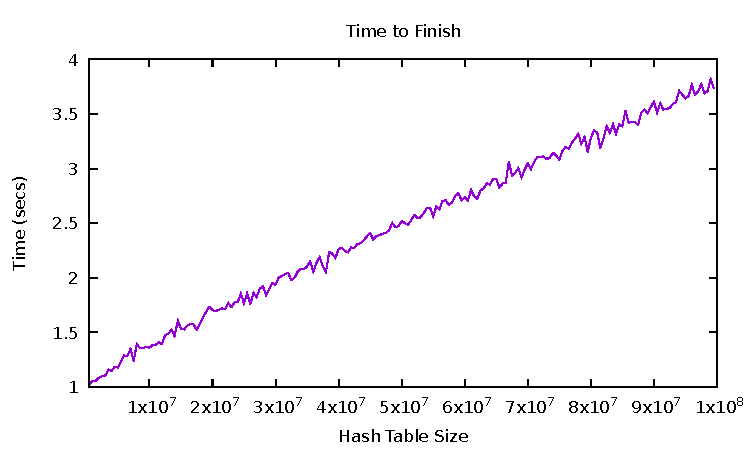
\includegraphics{plots/big-ht-time.pdf}\caption{The correlation between hash table size and program speed}
\end{centering}\end{figure}

However, if we zoom into the smaller hash table sizes and plot the time logarithmically (for visibility), we can see an interesting pattern emerge at the small values. Up to an array of about $10^6$ elements, the speed stays about the same. However, after that point, the time begins to rise more rapidly. This is due to the faster L3 cache, which seems to be sized at around 8 MB (1 million-index array of 8-byte pointers).

\begin{figure}[H]\begin{centering}
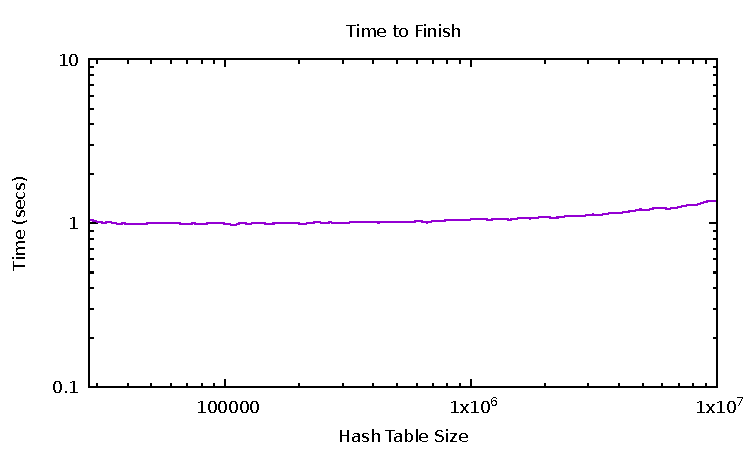
\includegraphics{plots/small-ht-time.pdf}\caption{Hash table size vs time on a smaller scale}
\end{centering}\end{figure}

But wait, what's that at the start? If we look closely, we can see a slight curve downwards. This is most likely because of an increase in the number of hash table collisions and therefore linear probing. Let us zoom in to that section further, and turn our focus more to the nature of hash tables.

\section{Hash Table Collisions}
If we zoom into the start of the graph even more, we see something interesting happen: the very start is actually a bit slower! The starting hash table size was found by testing the text inputs and finding the minimum size for the hash table not to fill completely, which turned out to be exactly 27122. It is then seen that the program speed with that size is slow. We ask ourselves: why is it slow? Let us consider the hash table insertion and lookup algorithms. If we are inserting a value and have a collision (the intended spot of the hash is full), we move along the hash table until we find an open spot. With an array that's just large enough to hold all the words, there will be many collisions, and worst-case an insertion will have to probe 27120 more times before finding the last open spot. The same happens with our lookups: we have to scan more and more indices as the hash table approaches its limit. Therefore, the inefficiency of our linear insertions and lookups outweighs the size of the array, leading to a less efficient program.

\begin{figure}[H]\begin{centering}
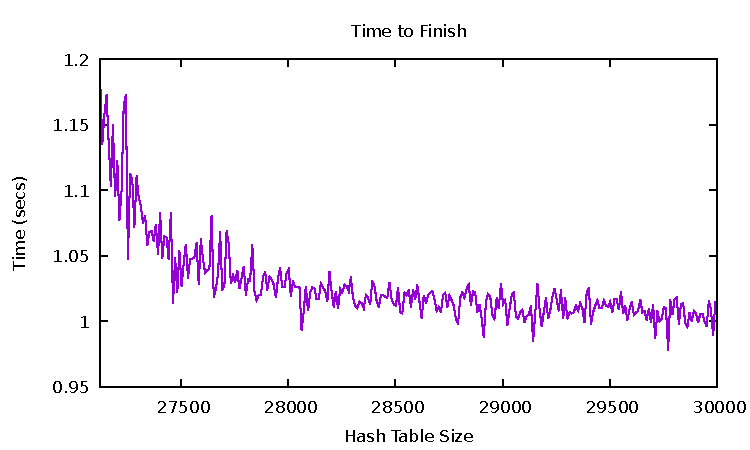
\includegraphics{plots/smallest-ht-time.pdf}\caption{Hash table size vs time at the smallest sizes}
\end{centering}\end{figure}

This leads us to our next question: there must be a point at which the program is most efficient; where the size of the hash table does not slow the program down and nor does the number of collisions. Of course, the size of the table will depend on the texts being given to the program: Shakespeare alone contains over 45,000 unique non-noise words. We can approximate this value for the data set we have been already using by sorting our data to bring out the lowest value. Using the command \verb|$ sort -n -t ' ' -k 2 < times.dat|, we can sort the data as needed and see the fastest times. While there is no clear and exact pattern, it is visible that all program runs under 1 second had a hash table size of 250,000 or less, and most were under 100,000; therefore, we can deduce that it is a good idea to keep the size of the hash table at around 5x the size of the largest text to minimize collisions. Of course, this may change at a size of $10^6$ as we move from the L3 cache to DRAM, but we do not currently have a data set to test that properly.

\section{Compilation Optimization}
When I first built my program, the only flags I used for compilation were\\\verb|-Wall -Wextra -Werror -Wpedantic|, as instructed. However, when I complained about the program running 4 times slower than the example binary, Eugene recommended I use \verb|-Ofast|. After adding this flag to my compilation flags, the program sped up to match the example. One must wonder: what changed in the code to allow for this massive optimization? We use \verb|gprof| to analyze the functions taking up the most time in each program:
\newpage
Unoptimized program:
\begin{verbatim}
% time  seconds   seconds    calls  Ts/call  Ts/call  name    
 66.50     13.32    13.32                             hash
  5.79     14.48     1.16                             ht_iter
  5.29     15.54     1.06                             ht_insert
  3.69     16.28     0.74                             bv_get_bit
  3.05     16.89     0.61                             text_create
\end{verbatim}
Optimized program:
\begin{verbatim}
% time  seconds   seconds    calls  Ts/call  Ts/call  name    
 53.74      4.53     4.53                             hash
 10.32      5.40     0.87                             ht_insert
  7.83      6.06     0.66                             bv_get_bit
  5.69      6.54     0.48                             ht_lookup
  4.51      6.92     0.38                             text_create
\end{verbatim}
We can see that essentially the same five functions are taking up the most time, especially the hash function. However, the optimized hash function is the most greatly pronounced optimization of them all, with the time taken decreased by almost three times. It is even visible that the hash function only takes 54\% of the optimized program's time but 67\% of the unoptimized program's time. All the other functions also have increased efficiency if we look at the seconds taken by each, though not nearly as much as the hash function.

Now sure, we've rambled on about the program's efficiency, but let us actually take a look at what is happening here. Since the biggest optimizations came from the hash function, we will inspect its object file and the produced assembly code, using \href{https://godbolt.org/z/xafdr34hc}{Godbolt} to do so as recommended by Ben. Immediately, it is apparent that the optimized assembly code is shorter, reaching only 57 lines vs the unoptimized 84. It is also very interesting to see how split and unorganized the optimized code is compared to the unoptimized code, with the unoptimized code keeping each line of code's instructions in order. This makes sense, of course, but it almost seems like the optimized code is trying to do more things at once despite the program being linear. The root calls are still there of course, and in order, but many of the \verb|ldr| calls are replaced with \verb|mov|, and many of them are just missing. It's very interesting to see the \verb|bl strlen| call, the underlying \verb|ble| (branch if less than or equal to) calls that make up the \verb|for| loop, and how it's laid out in assembly code. Much of it is beyond my understanding unfortunately, but it was still interesting to see the role that the compiler plays in the robustness and performance of the program.

\section{Bloom Filters}
The Bloom filter served as our first layer of ``defense" when checking for the existence of a word in a text. After checking the filter, we attempted to find the word in the hash table to rule out any false positives. While this would normally be a good way to check, the slowness of the hashing function actually makes the Bloom filter a slowdown compared to the hash table. The linear probing of the hash table is almost always faster than hashing the three indices for the Bloom filter. However, there are some changes that go along with the size of the filter, as seen below.

\begin{figure}[H]\begin{centering}
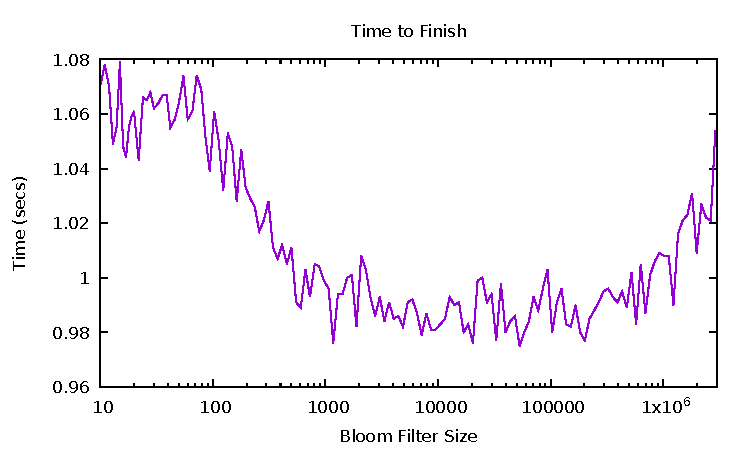
\includegraphics{plots/bf-time.pdf}\caption{Bloom filter size vs program runtime}
\end{centering}\end{figure}

Clearly, there is some sort of middle ground to be found for the Bloom filter. When the size is very small, the filter servers very little purpose as they provide an overwhelming number of false positives (covered later). However, when the filter gets too large, the memory required for the array becomes unwieldy for the program. As seen in the plot, there is a middle ground in-between, at a size of around 25,000.

Let us now look at the aforementioned false positive count. The following plot shows the downwards trend of false positives in the Bloom filter as the size increases. However, there is very little gain to expanding the graph past around 10,000 or so, as the increased size does not decrease collisions by much.

\begin{figure}[H]\begin{centering}
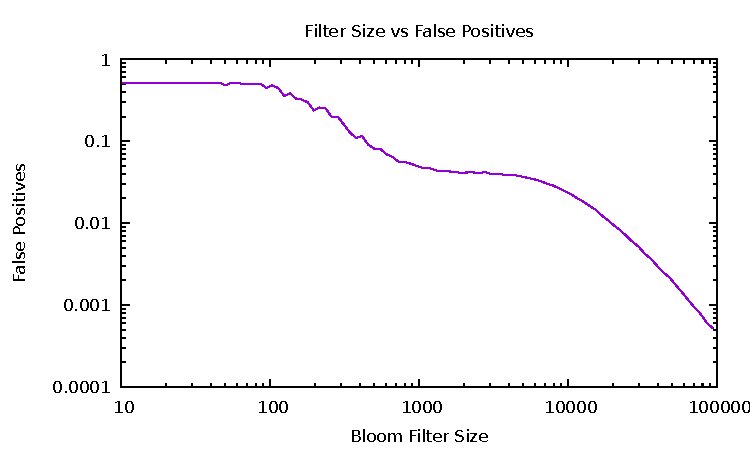
\includegraphics{plots/false-positives.pdf}\caption{Bloom filter size vs false positives}
\end{centering}\end{figure}

These numbers and takeaways are obviously dependent on the size of the input texts, as the ones used here only contain around 27,000 unique words. We can see that the optimal Bloom filter size is around the same as the number of unique words in the texts. However, the Bloom filters are actually pretty useless here. If we remove the Bloom filters from use completely, we can see that our program speeds up by 1.5 times. This is due to the painfully slow hash function being the biggest roadblock in the program.
\begin{verbatim}
Full Database Run
With Bloom Filter: 14.252s
Average Probes per Lookup: 1.004418
Without Bloom Filter: 9.867s
Average Probes per Lookup: 1.003461
\end{verbatim}
Despite the optimizations we have made, it is clear that we are better off without the Bloom filter. The average probes per lookup is lower because we probe the hash table for nodes we could have found were empty through the Bloom filter, but we have more probes in total. However, this does not allow us to optimize the program, as again, the hash function is the limiter.

\section{Distance Formulae}
When comparing the three distance formulas used, it is interesting to note the similarities and differences between the results. Euclidean and Manhattan distance both provide a distance of 0 for the exact text, while Cosine distance provides all results slightly under 1. The Cosine distance also shows some very different results compared to the results of the Euclidean and Manhattan distances. One must wonder: what makes each function different? The Euclidean and Manhattan distances are similar since they use the absolute value of the difference in both cases, but the Manhattan distance uses a Pythagorean-theorem-like formula to find the distance. The Cosine distance, however, utilizes multiplication to find the distance. When two frequent appearances are multiplied together, the product is larger than if a small value and a large value are multiplied together, or especially when one of the frequencies is 0. Subtracting 1 afterwards simply allows us to label the closest ones as smallest and utilize our priority queue.

\section{Conclusion}
This assignment showcased some interesting ways to keep a set of values ordered in a unique way using their keys. Bloom filters, hash tables, and a hashing algorithm worked together to create a relatively efficient storage and lookup method for our texts, and the texts served as a layer of abstraction to create and compare the distances between vectors. This also allowed me to gain insight into the world of similarity and plagiarism checking, and cleared up some of the mysticism of that topic.
\end{document}
